\begin{figure}[H]
	\begin{center}
		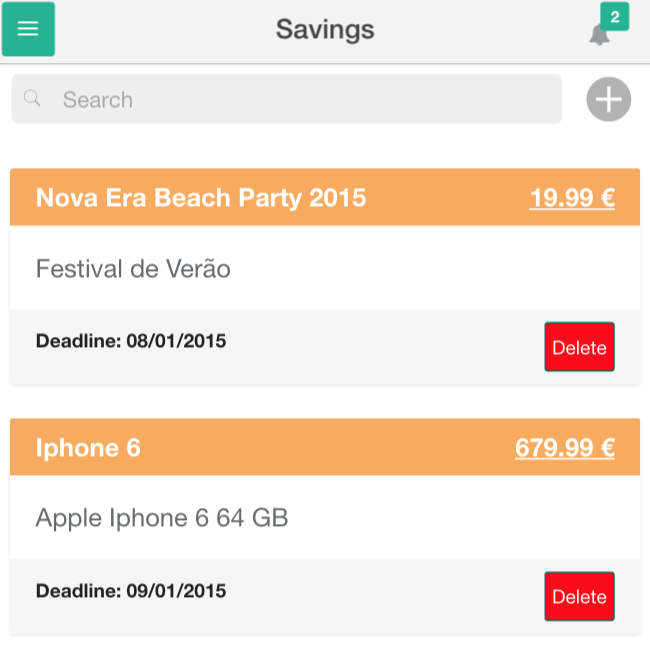
\includegraphics[width=0.5
		\textwidth]{savings/savings.png}
	\end{center}
	\caption{Poupanças Ativas}
	\label{fig:7}
\end{figure}

As poupanças são metas que o utilizador pretende alcançar e são constituídas por uma data limite, um montante e a descrição da poupança. A Figura \ref{fig:7} apresenta a lista de poupanças do utilizador.

\begin{figure}[H]
	\begin{center}
		\includegraphics[width=0.5
		\textwidth]{savings/addSavings.png}
	\end{center}
	\caption{Adicionar Poupança}
	\label{fig:7_1}
\end{figure}

Para adicionar uma nova poupança seleciona-se o botão de adicionar presente no ecrã de lista de poupanças. Surge um novo ecrã onde é necessário preencher todos os dados referentes à poupança.